%
%Free under Creative Commons Attribution-NonCommercial 4.0 International (CC BY-NC 4.0)
%


\documentclass[12pt]{article}
\usepackage{fancyhdr}
\usepackage{color}
\usepackage{multicol}
\usepackage{enumitem}
\usepackage{graphicx}
\usepackage{sectsty}
\usepackage{amsmath}
\usepackage{amssymb}
\usepackage{hyperref}
\usepackage{array}
\usepackage{scrextend}
\usepackage{blindtext}
\usepackage[first=-100, last=100]{lcg}

\newcommand{\sectionbreak}{\clearpage}

\usepackage{tikz}
	\usetikzlibrary{arrows,shapes,trees}

\usepackage{tkz-euclide}
\usetkzobj{all}

\allsectionsfont{\centering}

\usepackage{draftwatermark}
	\SetWatermarkText{wolf-math.com}
	\SetWatermarkScale{5}
	\SetWatermarkAngle{90}
	\SetWatermarkLightness{1}

\usepackage[margin=1in, headsep=0pt]{geometry}
\setlength{\parindent}{0cm}
\pagestyle{empty}

\begin{document}
\newcommand{\random}{\rand\arabic{rand}}



Mr. Wolf\\
wolf-math.com\\

\section{Lesson Plan -- Sequences and Series}


\subsection{Goals \& Objectives}

\begin{enumerate}

\item \textbf{SWBAT} identify arithmetic sequences 

\item \textbf{SWBAT} identify geometric sequences 

\item \textbf{SWBAT} determine the $n^{th}$ term of a sequences

\item \textbf{SWBAT} determine the rule of a sequence

\item \textbf{SWBAT} use proper sequence notation

\item \textbf{SWBAT} use $\Sigma$ notation for series

\item \textbf{SWBAT} find the sum of a series

\end{enumerate}

\subsection{Standards}

\textbf{Interpreting Functions } \hfill F-IF\\

Understand the concept of a function and use function notation\\

3.	 Recognize that sequences are functions, sometimes defined
recursively, whose domain is a subset of the integers. For example, the
Fibonacci sequence is defined recursively by $f(0) = f(1) = 1$, $f(n+1) = f(n) +
f(n-1)$ for $n ≥ 1$.\\

\textbf{Building Functions 	\hfill F-BF}\\

Build a function that models a relationship between two quantities\\

2.	 Write arithmetic and geometric sequences both recursively and
with an explicit formula, use them to model situations, and translate
between the two forms. \\

\textbf{Linear and Exponential Models ★ \hfill 	F-LE}\\

Construct and compare linear and exponential models and solve
problems\\

2.	 Construct linear and exponential functions, including arithmetic and
geometric sequences, given a graph, a description of a relationship, or
two input-output pairs (include reading these from a table).\\

\subsection{Connections}

\textbf{Now} we are learning about how patterns arise in mathematics.\\

\textbf{Later} we will learn about functions; how they are similar or different from sequences.\\

\let\stdsection\section
\renewcommand\section{\newpage\stdsection}

%\begin{addmargin}[4em]{1em}
%\end{addmargin}

\section{Sequences}

A \textbf{Sequence} is a list of things.\\

\subsection{Sequence Activity}

\begin{enumerate}

\item Make a list of pictures, numbers, or letters.

\item Circle the second term.

\item What rules does your sequence follow?	

\item Is your sequence an infinite sequence, or is it finite?

\item Could you change the -finity of your sequence?

\end{enumerate}

So, as identified from the activity, a sequence is any list or progression of things. Usually sequences are numbers, but they can really be anything. \\

\textbf{Examples:}\\

\begin{addmargin}[4em]{1em}

$\{1,2,3,4,5,6,....,n\}$ -- counting up by 1.\\

\{c, d, e, f, g, ...\} -- The alphabet starting at "c."\\

$\{1,0,8,08,88...\}$ -- the number of close spaces in each term.\\

\{M, C, 2, S, T, E, M\} -- School name\\

$\{6,5,4,3\}$ -- Count backwards from 6 to 3.\\

$\{1,2,1,2,1,2,1,...\}$ -- Alternate 1, 2.

\end{addmargin}

\subsection{-Finity}

Some sequences are infinite and other are finite. When listing a sequence infinity is determined by 3 dots at the end. $\{1,2,3,...\}$. If it doesn't have 3 dots we assume it's finite. If we're using a mathematical formula (see \ref{Formulas}) we assume that it's infinite and it follows the mathematical rule forever.

\subsection{Notation}

Sequences have curly brackets around them, \{\}, and commas between the elements. Each element of the sequence is called a \textbf{term}. Sometimes they are called "elements", or "members."\\

Formulas are written with subscript. $a_n$. The title of the sequence is $a$, and $n$ is the term number. $a_n$ is the value of the term number.\\

\begin{addmargin}[4em]{1em}

	Example:	$a_n=3n+2$\\
	
				$$a_1=3(1)+2=5$$
				$$a_2=3(2)+2=8$$
				$$a_3=3(3)+2=11$$
				$$\vdots$$
				
			So, $a_n=3n+2=\{5,8,11,...\}$

\end{addmargin}


\subsection{Formulas}

It's best to determine the formula for a sequence.\\

Take $\{3,5,7,9,...\}$, \ it's ok to say "start on 3 and add 2," but that makes it difficult to figure out the 823$^{rd}$ term.  So we should determine a mathematical formula. Different types of sequences have different ways of determining the formula. We will see them each in a little bit.\\





\section{Arithmetic Sequence}

An \textbf{Arithmetic Sequence} is a pattern of numbers through addition or subtraction.\\

\textbf{ex 1)} $\{1,4,7,10,13,16,19,22,...\}$

This sequence begins on $1$ and increases by $3$ each term. If you subtract any term by the term that succeeds it you should get $3$. This number ($3$ in our example) is called the \textbf{common difference}.\\

We therefore could write a sequence as $\{a, a+d, a+2d, a=3d,...\}$\\, where $a$ is the first term and $d$ is the common difference. \\

\textbf{You Try:} Determine the sequences are arithmetic sequences. If so what's the common difference?\\

\begin{enumerate}
\item $\{2,7,12,17,22,...\}$\\
$d=$\\

\item $\{10,8,6,4,2,...\}$\\
$d=$\\

\item $\{1,2,4,8,16,32,64,...\}$\\
$d=$\\

\item $\{2,6,10,14,18,22,...\}$\\
$d=$\\

\item $\{27,9,3,1,...\}$\\
$d=$\\	
\end{enumerate}

\subsection{Writing Formulas for Arithmetic Sequences}

We use the general form $$a_n=a+d(n-1)$$ where $a$ is the first term and $d$ is the common difference. $(n-1)$ is used because $d$ is not in the first term.\\ 

Take our arithmetic sequences from the "you try." Just plug in and simplify\\

\bgroup
\def\arraystretch{2}%  1 is the default, change whatever you need
%\setlength{\tabcolsep}{.4in}
\begin{tabular}{l l l}
 $\{2,7,12,17,22,...\}$ & $d=5$ & $a_n=2+5(n-1)=5n-3$\\

 $\{10,8,6,4,2,...\}$ & $d=-2$ & $b_n=10-2(n-1)=-2n+12$\\

 $\{2,6,10,14,18,22,...\}$ & $d=4$ & $c_n=2+4(n-1)=4n-2$\\
\end{tabular}
\egroup

Another way to do this is $a_n=dn+(a-d)$, where $a$ is the first term and $d$ is the common difference. Both ways are acceptable.\\

\section{Summation of Arithmetic Sequences: Arithmetic Series}

We know that $a_n= a_1 , a_2 , a_3 , a_4 ...$ is a pattern that repeats at a constant rate. What if we wanted to add up all of these terms ($a_1+a_2+a_3...$)?\\

\begin{addmargin}[4em]{1em}

\textbf{Example:} The following pattern of a pyramid is demonstrated by arithmetic sequence $b_n=2n-1$\\

\begin{center}

\begin{tabular}{l c}

Step 1 & X\\
Step 2 & XXX\\
Step 3 & XXXXX\\
Step 4 & XXXXXXX\\
\vdots & \vdots

\end{tabular}

\end{center}

To figure out how many X's are on the $8^{th}$ level, we would plug in to the formula, $b_8=2(8)-1=15$. So there are 15 X's on the $8^{th}$ level. How many X's have been used total? All of the levels need to be added together to figure that out.\\

We'll come back to this in a minute.\\

\end{addmargin}

To indicate the \textbf{sum} of the terms of a sequence we use \textbf{sigma notation}.\\

$$\sum\limits_{i=1}^{n} a_n = a_1 + a_2 + a_3 + a_4 + a_5 + ...$$

The $\Sigma$ means that we are \textbf{adding} the parts of the pattern together. \\ 

$i$ is the \textbf{starting term} from where we will begin adding things together.\\

$n$ is the \textbf{ending term} from where we finish adding things together.\\


If we want to know how many X's are in the pyramid from $1^{st}$ term to the $8^{th}$ term we'd use $\Sigma$ notation to indicate that sum.\\

$$\sum\limits_{i=1}^{8}b_n$$

or since $b_n=2n-1$

$$\sum\limits_{i=1}^{8}2n-1$$

In either case it would be $1+3+5+7+9+11+13+15=64$\\

\pagebreak


\textbf{You Try:}

\begin{enumerate}
 
 \item $\sum\limits_{n=1}^{5} 2n =$
 
 \item $\sum\limits_{b=1}^{4} 2b-5 =$
 
 \item $\sum\limits_{g=3}^{10} 3g-1 = $\\
\end{enumerate}

$\sum\limits_{n=1}^{5} 2n = 2(1) + 2(2) + 2(3) + 2(4) + 2(5) = 2+4+6+8+10 = 30$\\

$\sum\limits_{b=1}^{4} 2b-5 = [2(1)-5] + [2(2)-5] + [2(3)-5] + [2(4)-5] = $\\

$\sum\limits_{g=3}^{10} 3g-1 = [3(3)-1] + [3(4)-1] +[3(5)-1] +[3(6)-1] +[3(7)-1] +[3(8)-1] +[3(9)-1] +[3(10)-1] =$\\

\vspace{.7in}

The opposite can also be done. How would the following sum be written in Sigma notation?

$5+9+13+17+21+25$\\

\begin{addmargin}[4em]{1em}

	Since $h_p=4p+1$, and since we are adding from the $1^{st}$ term to the $7^{th}$ term we write:

	$$\sum\limits_{p=1}^{7} 4p+1 $$

	or more simply (but less clearly ...

	$$\sum\limits_{p=1}^{7} h_p$$
\end{addmargin}

\textbf{YOU TRY:} Rewrite the following in sigma notation\\

$$1+3+5+7+9+11+13$$

BUT WAIT!!! There's a better way to do this. Let's look at the sum of all integers from 1 to 100. We could add $1+2+3+4+5+...+98+99+100$, but that's awfully long. Let's add two sums together (vertically) in opposite order and see what happens.

\begin{center}
\begin{tabular}{c c c c c c c c c c c c c}
1&+&2&+&3&+&...&+&98&+&99&+&100\\
+& & & & & & & & & & & &\\
100&+&99&+&98&+&...&+&3&+&2&+&1
\end{tabular}
\end{center}

What do each of these columns add up to? Each one of them adds up to 101, and there are 100 columns. So if we add all of these together we get 10100. But that's double the amount of the sum, so just divide by 2 and get 5050!\\

TL;DR: Add the first and last term, multiply by the number of terms, then divide by 2.\\

Or use this formula: $$\sum\limits_{i=1}^{k}a_n=\frac{k(a_1+a_k)}{2}$$ where $n=$ the number of terms\\ $a_1=$ the first term\\ $a_k=$ the last term.\\

For adding all the numbers from 1 to 100... $$\frac{100(1+100)}{2}$$\\

\begin{addmargin}[4em]{1em}

\textbf{You try:}\\

\begin{enumerate}

\item $\sum\limits_{i=1}^{10}2n+5$

\item $\sum\limits_{i=1}^{7}3n$

\item $\sum\limits_{i=4}^{11}6n-6$

\end{enumerate}

\end{addmargin}

\section*{Quiz Review: Arithmetic Sequences and Series}

Mr. Wolf \hfill NAME:\underline{\hspace{3in}}\\
2015-2016\\
$mc^2$ High School \hfill DATE:\underline{\hspace{2in}}\\

Determine whether or not the following are arithmetic sequences.\\

\begin{enumerate}
\begin{multicols}{2}
\setlength\itemsep{1cm}

	\item $1,2,3,4,...$\\
	
	\item $4,3,2,1,...$\\
	
	\item $10,1,8,2,7,3,...$\\
	
	\item $3,9,27,...$\\

\end{multicols}
\end{enumerate}

Determine the \textbf{common difference} of the sequence.\\


\begin{enumerate}[resume]
\begin{multicols}{2}
\setlength\itemsep{1cm}

	\item $9,5,1,-3,...$\\
	
	\item $2,5,8,11,...$\\
	
	\item $100,150,200,250,...$\\
	
	\item $25,-2,-29,-56,...$\\

\end{multicols}
\end{enumerate}

Create a formula for the sequence. $a_n=dn+(a_1-d)$ or $a_n=a_1 + d(n-1)$\\


\begin{enumerate}[resume]
\begin{multicols}{2}
\setlength\itemsep{1cm}

	\item $1,3,5,7,9,...$\\
	
	\item $2,-4,-10,-16,...$\\
	
	\item $7,10,13,16,...$\\
	
	\item $-10,-16,-22,-28,...$\\

\end{multicols}
\end{enumerate}

Calculate the value for $n$\\

\begin{enumerate}[resume]
\begin{multicols}{2}
\setlength\itemsep{1cm}

	\item $a_n=7n+13$, $n=10$
	
	\item $b_n=-9n+100$, $n=10$
	
	\item $c_n=5n-12$, $n=6$
	
	\item $d_n=4n-4$, $n=4$

\end{multicols}
\end{enumerate}

\pagebreak

Find the $n^{th}$ term of the sequence.\\

\begin{enumerate}[resume]
\begin{multicols}{2}
\setlength\itemsep{1cm}

	\item $a_1=4$, $d=3$, $n=30$\\
	
	\item $a_1=-52$, $d=10$, $n=17$\\
	
	\item $a_1=-6$, $d=13$, $n=32$\\
	
	\item $a_1=-10$, $d=3$, $n=15$\\

\end{multicols}
\end{enumerate}

Evaluate the arithmetic series. Use any method we learned to find the sum.\\

\begin{enumerate}[resume]
\begin{multicols}{2}
\setlength\itemsep{1.5cm}

	\item $\sum\limits_{i=1}^{10} 2n-1=$\\
	
	\item $\sum\limits_{i=1}^{25} 5n =$\\
	
	\item $\sum\limits_{i=1}^{40} -4n+44$\\
	
	\item $\sum\limits_{i=1}^{55} 3n-27$\\

\end{multicols}
\end{enumerate}

Evaluate the arithmetic series.\\

\begin{enumerate}[resume]
\begin{multicols}{2}

	\item $a_1=10$, $a_n=19$, $n=3$\\
	
	\item $b_1=19$, $b_n=95$, $n=20$\\

\end{multicols}
\end{enumerate}

\vfill SCORE:\underline{\hspace{1in}}

\section*{Quiz Review 2: Arithmetic Sequences and Series}

Mr. Wolf \hfill NAME:\underline{\hspace{3in}}\\
2015-2016\\
$mc^2$ High School \hfill DATE:\underline{\hspace{2in}}\\

Determine whether or not the following are arithmetic sequences.\\

\begin{enumerate}
\begin{multicols}{2}
\setlength\itemsep{1cm}

	\item $2,4,6,8,...$\\
	
	\item $8,5,2,-1,...$\\
	
	\item $1,11,111,1111,11111,...$\\
	
	\item $4,4,4,...$\\

\end{multicols}
\end{enumerate}

Determine the \textbf{common difference} of the sequence.\\


\begin{enumerate}[resume]
\begin{multicols}{2}
\setlength\itemsep{1cm}

	\item $13,7,1,-5,...$\\
	
	\item $2,5,8,11,...$\\
	
	\item $10,13,16,19,...$\\
	
	\item $5,-2,-9,-16,...$\\

\end{multicols}
\end{enumerate}

Create a formula for the sequence. $a_n=dn+(a_1-d)$ or $a_n=a_1 + d(n-1)$\\


\begin{enumerate}[resume]
\begin{multicols}{2}
\setlength\itemsep{1cm}

	\item $-11,-13,-15,-17,-19,...$\\
	
	\item $5,-4,-13,-22,...$\\
	
	\item $0,3,6,9,...$\\
	
	\item $10,7,4,1,-2,...$\\

\end{multicols}
\end{enumerate}

Calculate the value for $n$\\

\begin{enumerate}[resume]
\begin{multicols}{2}
\setlength\itemsep{1cm}

	\item $a_n= \random n + \random$, $n= \random$
	
	\item $b_n= \random n + \random$, $n= \random$
	
	\item $c_n= \random n + \random$, $n= \random$
	
	\item $d_n= \random n + \random$, $n= \random$

\end{multicols}
\end{enumerate}

\pagebreak

Find the $n^{th}$ term of the sequence.\\

\begin{enumerate}[resume]
\begin{multicols}{2}
\setlength\itemsep{1cm}

	\item $a_1=2$, $d=3$, $n=15$\\
	
	\item $a_1=-42$, $d=18$, $n=16$\\
	
	\item $a_1=-8$, $d=12$, $n=17$\\
	
	\item $a_1=-13$, $d=5$, $n=13$\\

\end{multicols}
\end{enumerate}

Evaluate the arithmetic series. Use any method we learned to find the sum.\\

\begin{enumerate}[resume]
\begin{multicols}{2}
\setlength\itemsep{1.5cm}

	\item $\sum\limits_{i=1}^{10} 5n-25=$\\
	
	\item $\sum\limits_{i=1}^{25} 6n-12 =$\\
	
	\item $\sum\limits_{i=1}^{100} -4n+44$\\
	
	\item $\sum\limits_{i=1}^{250} n-250$\\

\end{multicols}
\end{enumerate}

Evaluate the arithmetic series.\\

\begin{enumerate}[resume]
\begin{multicols}{2}

	\item $a_1=60$, $a_n=810$, $n=11$\\
	
	\item $b_1=-9$, $b_n=81$, $n=11$\\

\end{multicols}
\end{enumerate}

\textbf{Accelerated Objectives:} Evaluate the series.

\begin{enumerate}[resume]
\setlength\itemsep{1.7cm}

	\item $-7-2+3+8...88$\\
	
	\item The sum of an arithmetic series is $374$. If $a_1=-2$, and $d=3$, how many terms are being added together?

\end{enumerate}

\vfill SCORE:\underline{\hspace{1in}}

\section*{Quiz -- Arithmetic Sequences \& Series}

Mr. Wolf \hfill NAME:\underline{\hspace{3in}}\\
2015-2016\\
$mc^2$ High School \hfill DATE:\underline{\hspace{2in}}\\

Determine whether or not the following are arithmetic sequences.

\begin{enumerate}
\begin{multicols}{2}
\setlength\itemsep{1.2cm}

	\item $1,3,5,7,...$\\
	
	\item $10,7,4,1,...$\\
	
	\item $1,20,300,4000,50000,...$\\
	
	\item $4,5,4,5,...$\\

\end{multicols}
\end{enumerate}

Determine the \textbf{common difference} of the sequence.


\begin{enumerate}[resume]
\begin{multicols}{2}
\setlength\itemsep{1.2cm}

	\item $14,8,2,-4,...$\\
	
	\item $1,4,7,10,...$\\
	
	\item $12,15,18,21,...$\\
	
	\item $9,2,-5,-12,...$\\

\end{multicols}
\end{enumerate}

Create a formula for the sequence. $a_n=dn+(a_1-d)$ or $a_n=a_1 + d(n-1)$


\begin{enumerate}[resume]
\begin{multicols}{2}
\setlength\itemsep{1.2cm}

	\item $-2,-4,-6,-8,-10,...$\\
	
	\item $4,-4,-12,-20...$\\
	
	\item $1,2,3,4,...$\\
	
	\item $0,-2,-4,-6,...$\\

\end{multicols}
\end{enumerate}

Calculate the $n^{th}$ term.

\begin{enumerate}[resume]
\begin{multicols}{2}
\setlength\itemsep{1.2cm}

	\item $a_n=11n+2$, $n=7$
	
	\item $b_n=-6n+10$, $n=20$
	
	\item $c_n=9n-90$, $n=5$
	
	\item $d_n=4n-3$, $n=15$

\end{multicols}
\end{enumerate}

\pagebreak

Find the $n^{th}$ term of the sequence.

\begin{enumerate}[resume]
\begin{multicols}{2}
\setlength\itemsep{1.2cm}

	\item $a_1=12$, $d=13$, $n=5$\\
	
	\item $a_1=-4$, $d=1$, $n=6$\\
	
	\item $a_1=-28$, $d=2$, $n=13$\\
	
	\item $a_1=-12$, $d=6$, $n=12$\\

\end{multicols}
\end{enumerate}

Evaluate the arithmetic series. Use any method we learned to find the sum.

\begin{enumerate}[resume]
\begin{multicols}{2}
\setlength\itemsep{1.5cm}

	\item $\sum\limits_{i=1}^{11} n-11=$\\
	
	\item $\sum\limits_{i=1}^{16} 8n-32 =$\\
	
	\item $\sum\limits_{i=1}^{100} -10n+100$\\
	
	\item $\sum\limits_{i=1}^{3} 2n-4$\\

\end{multicols}
\end{enumerate}

Evaluate the arithmetic series given the first and last terms.

\begin{enumerate}[resume]
\begin{multicols}{2}

	\item $a_1=18$, $a_n=54$, $n=20$\\
	
	\item $b_1=-17$, $b_n=68$, $n=5$\\

\end{multicols}
\end{enumerate}

\textbf{Accelerated Objectives:} Evaluate the series.

\begin{enumerate}[resume]
\setlength\itemsep{1.7cm}

	\item $-8-4+0+4+...+108$\\
	
	\item If $a_1=-1$, and $a_{10}=107$, what is the formula for $a_n$? What is the sum of the first $10$ terms?

\end{enumerate}

\vfill SCORE:\underline{\hspace{1in}}

\section*{Quiz:: -- Arithmetic Sequences \& Series}

Mr. Wolf \hfill NAME:\underline{\hspace{3in}}\\
2015-2016\\
$mc^2$ High School \hfill DATE:\underline{\hspace{2in}}\\

Determine whether or not the following are arithmetic sequences.

\begin{enumerate}
\begin{multicols}{2}
\setlength\itemsep{1.2cm}

	\item $-1,1,3,5,...$\\
	
	\item $2,4,6,8,...$\\
	
	\item $11,9,7,5,...$\\
	
	\item $3,2,3,2,...$\\

\end{multicols}
\end{enumerate}

Determine the \textbf{common difference} of the sequence.


\begin{enumerate}[resume]
\begin{multicols}{2}
\setlength\itemsep{1.2cm}

	\item $14,7,0,-7,...$\\
	
	\item $12,16,20,24,...$\\
	
	\item $1,5,9,13,...$\\
	
	\item $7,2,-3,-8,...$\\

\end{multicols}
\end{enumerate}

Create a formula for the sequence. $a_n=dn+(a_1-d)$ or $a_n=a_1 + d(n-1)$


\begin{enumerate}[resume]
\begin{multicols}{2}
\setlength\itemsep{1.2cm}

	\item $-1,-3,-5,-7,...$\\
	
	\item $5,-5,-15,-25,...$\\
	
	\item $1,2,3,4,...$\\
	
	\item $0,6,12,18,...$\\

\end{multicols}
\end{enumerate}

Calculate the $n^{th}$ term.

\begin{enumerate}[resume]
\begin{multicols}{2}
\setlength\itemsep{1.2cm}

	\item $a_n=11n+2$, $n=9$
	
	\item $b_n=-6n+10$, $n=28$
	
	\item $c_n=9n-90$, $n=6$
	
	\item $d_n=4n-3$, $n=16$

\end{multicols}
\end{enumerate}

\pagebreak

Find the $n^{th}$ term of the sequence.

\begin{enumerate}[resume]
\begin{multicols}{2}
\setlength\itemsep{1.2cm}

	\item $a_1=12$, $d=13$, $n=6$\\
	
	\item $a_1=-4$, $d=1$, $n=16$\\
	
	\item $a_1=-28$, $d=2$, $n=14$\\
	
	\item $a_1=-12$, $d=6$, $n=2$\\

\end{multicols}
\end{enumerate}

Evaluate the arithmetic series. Use any method we learned to find the sum.

\begin{enumerate}[resume]
\begin{multicols}{2}
\setlength\itemsep{1.5cm}

	\item $\sum\limits_{i=1}^{12} n-12=$\\
	
	\item $\sum\limits_{i=1}^{16} 4n-16 =$\\
	
	\item $\sum\limits_{i=1}^{200} -20n+200$\\
	
	\item $\sum\limits_{i=1}^{3} 5n-15$\\

\end{multicols}
\end{enumerate}

Evaluate the arithmetic series given the first and last terms.

\begin{enumerate}[resume]
\begin{multicols}{2}

	\item $a_1=-1$, $a_n=66$, $n=20$\\
	
	\item $b_1=-8$, $b_n=8$, $n=5$\\

\end{multicols}
\end{enumerate}

\textbf{Accelerated Objectives:} Evaluate the series.

\begin{enumerate}[resume]
\setlength\itemsep{1.7cm}

	\item $-2+14+30+46+...+110$\\
	
	\item If $a_1=8$, and $a_{10}=62$, what is the formula for $a_n$? What is the sum of the first $10$ terms?

\end{enumerate}

\vfill SCORE:\underline{\hspace{1in}}



\pagebreak

\section{Geometric Sequences}

A \textbf{Geometric Sequence} is a sequence that increases of decreases by multiplication\footnote{remember that dividing is the same as multiplying by a fraction} of a constant.\\

\begin{addmargin}[4em]{1em}

\textbf{Example:}

$$\{1,2,4,8,16,32,64,128,...\}$$

\end{addmargin}

The general form of a geometric sequence is $$\{a,a\cdot r, a\cdot r^2, a\cdot r^3, a\cdot r^4,...\}$$

where $a$ is the first term and $r$ is the common ratio (the number they're getting multiplied by.\\

For the above example $a=1$ because the first term is $1$, and $r=2$ because each term is being multiplied by $2$. So plugging into the formula we get

$$\{a,a\cdot r, a\cdot r^2, a\cdot r^3, a\cdot r^4,...\}$$
$$\{1,1\cdot 2, 1\cdot 2^2, 1\cdot 2^3, 1\cdot 2^4,...\}$$
$$\{1,2,4,8,16,...\}$$

\subsection{Writing Formulas for Geometric Sequences}

The general form for a geometric sequence is $x_n=ar^{(n)}$. $a_1$ is the first term.

\textbf{Example:}\\

$$10, 30, 90, 270, 810, 2430, ...$$

$a_1=10$ and $r=3$\\

So, $$a_n=10\cdot 3^{(n)}$$

$\therefore$ $$ a_{10}=10\cdot 3^{(10-1)}=10 \cdot 3^9 = 10 \cdot 19683 = 196830$$

Geometric sequences can also get smaller by multiplying by a fraction or a decimal. For example, $$b_n=4,2,1,\frac{1}{2},\frac{1}{4},\frac{1}{8},...$$

The common ratio $r=\frac{1}{2}$\\

the first term $a_1=4$\\

So we can make our formula $b_n=4\cdot \left(\frac{1}{2}\right)^{n}$\\

\textbf{Be careful}  that $r\neq 0$. If $r=0$ then it's not a geometric sequence.\\


\section{Geometric Series}

Since the geometric sequence $$a_n= \{a_1, a_1 \cdot r, a_1 \cdot r^2, a_1 \cdot r^3, ...\}$$

then $$\sum\limits_{k=0}^{n-1}(a_1)= a_1 + a_1 \cdot r + a_1 \cdot r^2 + a_1 \cdot r^3 + ... + a_1 \cdot r^{(n-1)}$$

Just like with arithmetic series, the geometric series can be summed up with its own equation equation, $$\sum\limits_{k=0}^{n-1}a_1 \cdot r^{n-1}=a\left(\frac{1-r^n}{1-r}\right)$$


\section*{Exponential Functions}


\subsection*{Goals}

\textbf{SWBAT} identify exponential functions, and differentiate between exponential and power functions.\\

\textbf{SWBAT} graph exponential functions by using a t-chart.\\

\textbf{SWBAT} graph exponential functions without using a t-chart.\\

\textbf{SWBAT} determine the end behavior of an exponential function.\\

\textbf{SWBAT} identify translations of the exponential graph by identifying key parts of the equation.\\

\textbf{SWBAT} calculate compound interest given the interest rate, number of years, and number of times per year, and the principal.\\

\textbf{SWBAT} use the number $e$ as an exponential base for continuously compounded interest.\\



\subsection*{Standards}

\textbf{Creating Equations A -CED} Create equations that describe numbers or relationships\\

1. Create equations and inequalities in one variable and use them to solve problems. Include equations arising from linear and quadratic functions, and simple rational and exponential functions.\\

\textbf{Interpreting Functions F-IF} Analyze functions using different representations \\

7. Graph functions expressed symbolically and show key features of the graph, by hand in simple cases and using technology for more complicated cases.\\

e. Graph exponential and logarithmic functions, showing intercepts and end behavior, and trigonometric functions, showing period, midline, and amplitude.\\



\pagebreak

\section*{Introduction to Exponential Functions}

An exponential function is whenever there is a variable in the exponent. This is different from a power function where there is a variable with a rational number exponent.\\

Compare Linear vs. Power vs. Exponential functions\\

\begin{multicols}{3}
\begin{center}

\textbf{Linear}\\

{\renewcommand{\arraystretch}{2}
\begin{tabular}{c | c}

	$x$  & $y=2x$ \\ \hline
	0 & 0 \\
	1 & 2 \\
	2 & 4 \\
	3 & 6 \\
	4 & 8 \\
	5 & 10 \\
	\vdots & \vdots

\end{tabular}} \quad

\columnbreak

\textbf{Power}\\

{\renewcommand{\arraystretch}{2}
\begin{tabular}{c | c}

	$x$ & $y=x^2$ \\ \hline
	0 & 0 \\
	1 & 1 \\
	2 & 4 \\
	3 & 9 \\
	4 & 16 \\
	5 & 25 \\
	\vdots & \vdots

\end{tabular}} \quad

\columnbreak

\textbf{Exponential}\\

{\renewcommand{\arraystretch}{2}
\begin{tabular}{c | c}

	$x$ & $y=2^x$ \\ \hline
	0 & 1 \\
	1 & 2 \\
	2 & 4 \\
	3 & 8 \\
	4 & 16 \\
	5 & 32 \\
	\vdots & \vdots

\end{tabular}} \quad

\end{center}
\end{multicols} 

Notice that \textit{linear functions} always increase by the same amount by \textbf{addition}, \textit{Power functions} always increase by the \textit{square} of a number, and \textit{Exponential Functions} always increase by \textbf{multiplying} by the same amount.\\

\textbf{Example 2:} Determine which each chart represents: linear, power, or exponential.\\

\begin{multicols}{3}
\begin{center}



{\renewcommand{\arraystretch}{2}
\begin{tabular}{c | c}

	$x$  & $y=2x^3$ \\ \hline
	-2 & -16 \\
	-1 & -2 \\
	0 & 0 \\
	1 & 2 \\
	2 & 16 \\
	3 & 54 \\
	\vdots & \vdots

\end{tabular}} \quad

\columnbreak



{\renewcommand{\arraystretch}{2}
\begin{tabular}{c | c}

	$x$ & $y=2x-3$ \\ \hline
	-2 & -7 \\
	-1 & -5 \\
	0 & -3 \\
	1 & -1 \\
	2 & 1 \\
	3 & 3 \\
	\vdots & \vdots

\end{tabular}} \quad

\columnbreak



{\renewcommand{\arraystretch}{2}
\begin{tabular}{c | c}

	$x$ & $y=2 \cdot 3^x$ \\ \hline
	-2 & $\frac{2}{9}$ \\
	-1 & $\frac{2}{3}$ \\
	0 & 2 \\
	1 & 6 \\
	2 & 18 \\
	3 & 54 \\
	\vdots & \vdots

\end{tabular}} \quad

\end{center}
\end{multicols} 

\section*{Determine an Exponential Function from a Chart}

\begin{center}
{\renewcommand{\arraystretch}{2}
\begin{tabular}{c|c|c|c|c|c|c}

$x$ & -1 & 0 & 1 & 2 & 3  & ...\\ \hline
$y$ & $\frac{1}{10}$ & 1 & 10 & 100 & 1000 & ...\\ 

\end{tabular}} \quad
\end{center}

The rule for this chart is easy to determine. Since each $x$ increases the $y$ value by multiplying $10$, the equation is therefore $$y=10^x$$

But what about this...\\

\begin{center}
{\renewcommand{\arraystretch}{2}
\begin{tabular}{c|c|c|c|c|c|c}

$x$ & -1 & 0 & 1 & 2 & 3 & ... \\ \hline
$y$ & $\frac{11}{10}$ & 2 & 11 & 101 & 1001 & ... \\ 

\end{tabular}} \quad
\end{center}

The pattern goes away! There is no number to multiply by to get the next term. For this one we need to look at the first chart from $y=10^x$. Notice that the $y$ term for the second chart is always $1$ more than the $y$ value of the first chart. Besides that everything is the same.\\



%Do next: How to find the nth term! 

\pagebreak


\section*{Graphing Exponential Functions}

$$a\cdot b^{x-h}+k$$

The size of the base affects the vertical stretch of the function.\\

Compare $f(x)=2^x$ and $g(x)=3^x$

\begin{center}
\begin{tabular}{ l | c | c | c | c }
  \textbf{$x$} & $f(x)=2^x$ & \hspace{1cm} & $g(x)=3^x$ \\ \hline
  $-2$ & $\frac{1}{4}$ & & $\frac{1}{9}$\\ \hline
  $-1$ & $\frac{1}{2}$ & & $\frac{1}{3}$\\ \hline
  0  & 1 & & 1\\ \hline
  1  & 2 & & 3\\ \hline
  2  & 4 & & 9\\ \hline
  3  & 8 & & 27\\ \hline
  4  & 16 & & 81\\ \hline
  5  & 32 & & 243\\ \hline
  6  & 64 & & 729\\ \hline
  \vdots & \vdots & &\vdots
\end{tabular}
\end{center}

\begin{center}
%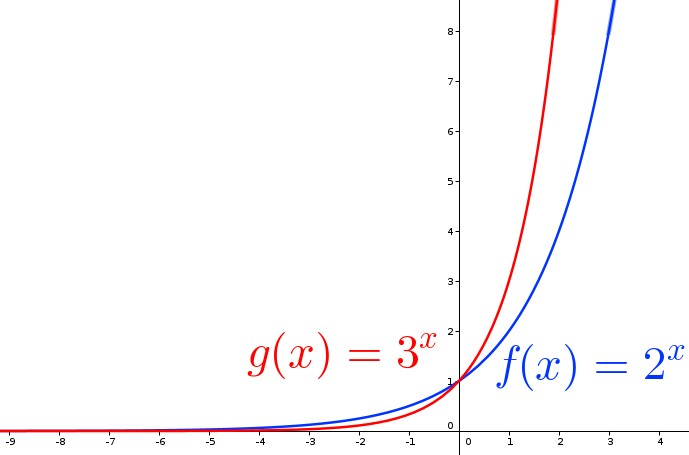
\includegraphics[scale=.5]{exponential.jpg}
\end{center}

Notice that the two functions overlap at $(0,1)$. Negative of here the larger base is smaller and the smaller base is bigger. Positive of here the larger base is bigger and the smaller base is smaller.\\

The two graphs will not go below the line $y=0$. This is called an \textbf{ASYMPTOTE}. It is a way of describing the \textit{end behavior} of a function. As the functions move towards negative infinity they will get smaller and smaller,  but they will never actually reach 0.\\

\pagebreak

\subsection*{Translations}

A translation is when a function is moved around the graph. To move the graph up or down, add or subtract from the function.

\begin{center}
%\includegraphics[scale=.5]{transformation1.jpg} 
\end{center}

If there is no $+h$ on the back of the function, then the asymptote is at $y=0$. In these cases the $h$'s are $+2$ and $-1$.\\

If there is a $+h$ or $-h$ then the asymptote is at $\pm h$\\

\hrulefill

To move the function side to side add or subtract from the exponent. Be careful because it goes in the opposite direction of the sign. Notice the asymptote doesn't move\\

\begin{center}
%\includegraphics[scale=.5]{transformation2.jpg}
\end{center}

\pagebreak

\section*{Method for Graphing}

Graph exponential equations. Easy method.

\begin{enumerate}
	\item Identify the asymptote. It's always the $\pm$ at the \textit{end} of the function
	
	\item Set the exponent equal to $0$
	
	\item Find the $y$ value when the exponent is equal to zero. Graph that point.
	
	\item Follow the asymtote until it passes through the point, and graph the exponentiality. \\
\end{enumerate}

\begin{multicols}{2}

\textbf{Example 1:} graph $y=2^{x-2}+3$\\

%%\includegraphics[scale=.75]{graphquads.jpg}\\

\textbf{Example 2:} graph $y=\left(\frac{1}{2} \right)^{x}-7$\\

%\includegraphics[scale=.75]{graphquads.jpg}\\

\textbf{Example 3:} graph $y=-2^{x-2}+3$\\

%\includegraphics[scale=.75]{graphquads.jpg}\\

\textbf{Example 4:} graph $y=2^{-x}-7$\\

%\includegraphics[scale=.75]{graphquads.jpg}\\

\end{multicols}

\pagebreak

\textbf{You Try:} Graph the exponential Functions\\

\begin{multicols}{2}
 $y=3^x-5$\\

%\includegraphics[scale=.8]{graphquads.jpg}\\

 $y=\left(\frac{1}{3} \right)^{x+4}+1$\\

%\includegraphics[scale=.8]{graphquads.jpg}\\

$y= (-2)3^{x-1}+6$\\

%\includegraphics[scale=.8]{graphquads.jpg}\\

$y= 3^{-x}$\\

%\includegraphics[scale=.8]{graphquads.jpg}\\




\end{multicols}

\pagebreak

\section*{Compound Interest}

Compounding interest is an exponential expression because the exponent changes as time goes on. \\


$$A=P(1+r)^t \hspace{1cm}  A=P\left(1+\frac{r}{n}\right)^{nt}$$\\

$A=$ Actual amount -- what you'll end up with

$P=$ Principle -- what you started with

$r=$ rate -- as a decimal, not as a fraction

$n=$ number of times per year

$t=$ time -- years\\

The \textit{independent} variable is $t$ the amount of time that goes by. The \textit{dependent} variable is the actual amount. This is because the actual amount depends on how much time goes by.\\ If we set this up as a relationship between $t$ and $A$, we would get an exponential function.

\hrulefill

\textbf{Example 1:}
How much will you have after investing \$500,000.00 compound yearly at 3\% for 12 years?\\


\vspace{1in}
\textbf{Example 2:}

How much will you have if you invest \$100 in a bond at \%5 compound monthly for 15 years.\\

\vspace{1in}

\textbf{Example 3:}
How much will you have after inveesting \$15.00 compound quarterly at 4\% since 1945 (the end of WW2)?\\

\pagebreak

\section*{Exponential (radioactive) Decay}

Exponential decay is the same as exponential growth except for a minus sign.\\

$$A=P(1-r)^t$$

\section*{The Number $e$}


e is an irrational number discovered by Leonhard Euler (pronounced oiler). It is commonly called Euler’s Number, but more commonly as the natural base. $e\approx 2.7182818...$ It is used as the base for many exponential functions, and has many applications in calculus.\\

$\mathbf{e}$ is calculated by the following expression as $n$ gets larger and larger $$\lim_{n \to \infty} \left(1+\frac{1}{n}\right)^n \approx 2.7182818$$\\

I hope this expression looks a little familiar.

\hrulefill

$e$ can be used a a regular exponential base. \\

So we can graph $y=e^x$\\

\begin{center}
%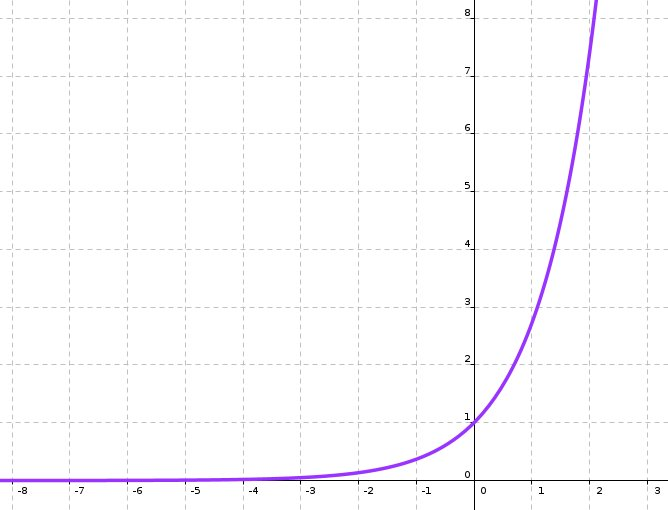
\includegraphics[scale=.75]{e.jpg}
\end{center}

What it comes down to is that $e$ is a number just like any other, and we can use it as such.\\

So what's so special about this number $e$?

\pagebreak

\section*{Continuously Compounded Interest}

What is so special about $e$ is that we can compound interest continuously. The nice thing about that is that I get more money when interest is compounded more frequently.\\

\begin{center}
%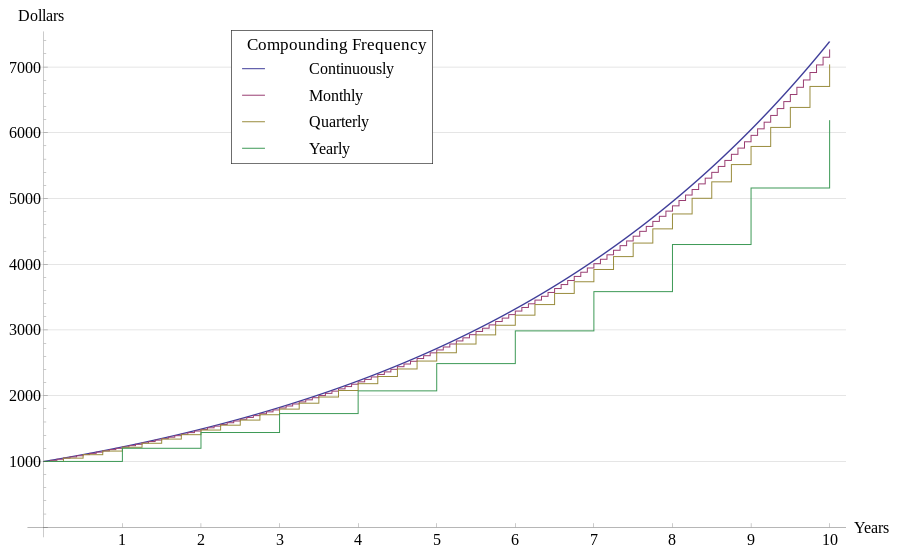
\includegraphics[scale=.5]{compoundinterest.png}
\end{center}

The graph above shows the same interest rate, but when the interest is compounded more often there are more significant gains made. \\

To calculate continuously compound interest we use the formula 

$$A=Pe^{rt}$$

Where\\
$A=$ Actualized amount\\
$P=$ Principal\\
$r=$ rate\\
$t=$ time\\

So basically all the letters are the same (remember $e$ is a number, not a variable), and it's a much tighter, neater package.\\

\pagebreak

\textbf{Example:} You deposit \$1500.00 in an account compound continuously at 3\%. How much will you have after 3 years?

\vspace{1in}

How much will you have after 10 years?\\

\vspace{1in}

How does this compare to compounded semi-annually (twice a year) for 10 years?\\

\vspace{1in}

\hrulefill

\textbf{Example 2:} How much will you have after investing \$2.00 compounded continuously since the year 1776?\\

\pagebreak

\section*{Quiz Review}

Mr. Wolf \hfill NAME:\underline{\hspace{3in}}\\ 
Pre-Calculus \\ 
$MC^2$ STEM HS \hfill DATE:\underline{\hspace{2in}}\\
2015-2016\\

\begin{center}
	\begin{Large}
		 Graphing Exponentials \& Exponential Growth\\

	\end{Large}
	
		\textbf{Due Monday} 2014-10-13\\
\end{center}


\textbf{Graph the exponential function}\\

\begin{enumerate}[resume]
\begin{multicols}{2}

\item graph $y=2^{x-2}+3$\\

%\includegraphics[scale=.65]{graphquads.jpg}\\

\item graph $y=\left(\frac{1}{2} \right)^{x}-7$\\

%\includegraphics[scale=.65]{graphquads.jpg}\\

\item graph $y=-2^{x-2}+3$\\

%\includegraphics[scale=.65]{graphquads.jpg}\\

\item  graph $y=2^{-x}-7$\\

%\includegraphics[scale=.65]{graphquads.jpg}\\

\end{multicols}

\end{enumerate}

\hrulefill

\textbf{Compound the Interest}\\

$$A=P\left(1+\frac{r}{n}\right)^{n \cdot t}$$

\begin{enumerate}[resume]

\item How much money would you have after investing \$17 compounded daily at 10\% for 25 years?\\

\item (Population Growth) A rabbit population increases at 60\% compounded quarterly. If there were 20 rabbits to start with, how many rabbits will there be after 10 years?\\

\item 	\begin{enumerate}

			\item How much would you have after investing \$400 compounded monthly at 5\% for 10 years?\\

			\item How much would you have after investing \$400 compounded monthly at 5\% for 20 years?\\
			
			\item Even though twice as much time went by between (a) and (b), was twice as much money made?\\

		\end{enumerate} 

\end{enumerate}

\hrulefill

\textbf{Continuously Compound Interest}\\

$$A=Pe^{rt}$$

\begin{enumerate}[resume]

\item How much money will you have after investing \$600 compounded continuously at 4\% for 8 years?\\

\vspace{1cm}

\item 	\begin{enumerate}
		
			\item How much money will you have if you invest \$500 compounded continuously at 12\% for 10 years?\\
			
			\item What's the difference between (a) and if you compounded twice per year for 10 years.\\
			
		\end{enumerate}

\end{enumerate}

\pagebreak

\section*{Quiz}

Mr. Wolf \hfill NAME:\underline{\hspace{3in}}\\ 
Pre-Calculus \\ 
$MC^2$ STEM HS \hfill DATE:\underline{\hspace{2in}}\\
2015-2016\\

\begin{center}
	\begin{Large}

		 Graphing Exponentials \& Exponential Growth\\

	\end{Large}
	
		\textbf{OPEN NOTE} \\
\end{center}


\textbf{Graph the exponential function}\\

\begin{enumerate}[resume]
\begin{multicols}{2}

\item graph $y=2^{x+2}-3$\\

%\includegraphics[scale=.65]{graphquads.jpg}\\

\item graph $y=\left(\frac{1}{2} \right)^{x}-8$\\

%\includegraphics[scale=.65]{graphquads.jpg}\\

\item graph $y=-2^{x+5}-3$\\

%\includegraphics[scale=.65]{graphquads.jpg}\\

\item  graph $y=2^{-x}+5$\\

%\includegraphics[scale=.65]{graphquads.jpg}\\

\end{multicols}

\end{enumerate}

\hrulefill

\textbf{Compound the Interest}\\

$$A=P\left(1+\frac{r}{n}\right)^{n \cdot t}$$

\begin{enumerate}[resume]

\item How much money would you have after investing \$17 compounded daily at 10\% for 25 years?\\

\item (Population Growth) A rabbit population increases at 60\% compounded quarterly. If there were 20 rabbits to start with, how many rabbits will there be after 10 years?\\

\item 	\begin{enumerate}

			\item How much would you have after investing \$1000 compounded monthly at 6\% for 10 years?\\

			\item How much would you have after investing \$1000 compounded monthly at 6\% for 30 years?\\
			
			\item Even though triple the time went by between (a) and (b), was triple the money made?\\

		\end{enumerate} 

\end{enumerate}

\hrulefill

\textbf{Continuously Compound Interest}\\

$$A=Pe^{rt}$$

\begin{enumerate}[resume]

\item How much money will you have after investing \$800 compounded continuously at 4\% for 6 years?\\

\vspace{1cm}

\item 	\begin{enumerate}
		
			\item How much money will you have if you invest \$1200 compounded continuously at 10\% for 14 years?\\
			
			\item What's the difference between (a) and compounded twice per year for 14 years.\\
			
		\end{enumerate}

\end{enumerate}

\vspace{1cm}

**Now you're done :-)
\end{document}